% \appendix
\chapter{Ejemplificación del bineado adaptativo}
\label{app:B}

En este apéndice se presenta una serie de ejemplos ilustrativos que permiten visualizar el funcionamiento del algoritmo de bineado adaptativo descrito en el Capítulo~\ref{cap:metodo_histogramas}. La variable seleccionada para la demostración es la \textit{letargía} de un archivo de partículas, que se presenta en la Figura~\ref{fig:B_letargia}. La distribución de letargía en este caso exhibe tres regiones distintivas:

\begin{figure}[H]
    \centering
    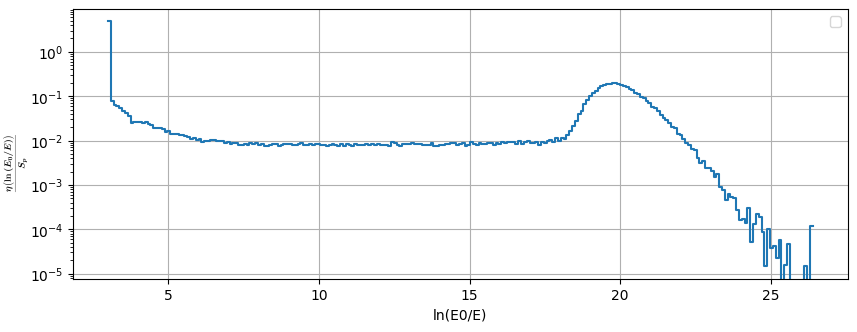
\includegraphics[width=\textwidth]{B_letargia.png}
    \caption{Distribución de letargía utilizada en la ejemplificación.}
    \label{fig:B_letargia}
\end{figure}

\begin{itemize}
    \item Una delta en $1~MeV$ asociada a una fuente monoenergética.
    \item Una región aproximadamente constante en la región epitérmico.
    \item Una acumulación en la región térmica.
\end{itemize}

Se parte de la distribución original de referencia, obtenida con alta resolución de bines, y se aplica el algoritmo de bineado adaptativo siguiendo el criterio de máxima discrepancia en la función de distribución acumulada (FDC). En cada iteración, se identifica el punto donde la diferencia absoluta entre la FDC original y la obtenida con el bineado actual es máxima, y se introduce allí un nuevo borde de bin. En este apendice se utiliza 1 bin como punto de partida, y se van añadiendo bines hasta alcanzar un total de 100 bines, lo que permite observar cómo el algoritmo refina la distribución a medida que se incrementa el número de bines.

En las siguientes secciones se presentan los resultados obtenidos para distintos números de bines: 1, 2, 3, 5, 10, 25 y 100. En cada caso, se muestran:

\begin{itemize}
    \item La distribución estimada con el bineado actual, comparada con la distribución de referencia.
    \item Las funciones de distribución acumulada (FDC) de ambas distribuciones.
    \item La diferencia absoluta entre ambas FDC, utilizada como criterio de refinamiento.
\end{itemize}

\section*{Caso con 1 bin}
\addcontentsline{toc}{section}{Caso con 1 bin}

En la Figura~\ref{fig:B_letargia_1} se muestra la distribución de letargía aproximada con un único bin. Dado que el histograma se construye con un único bin, representa el valor promedio de letargía sobre todo el dominio. En la Figura~\ref{fig:B_FDC_1} se presentan las FDCs de la distribución original de referencia y la obtenida con 1 bin, mientras que en la Figura~\ref{fig:B_FDCdiff_1} se muestra la diferencia absoluta entre ambas FDCs, que sirve como criterio para determinar la ubicación del nuevo bin en la siguiente iteración.

\begin{figure}[H]
    \centering
    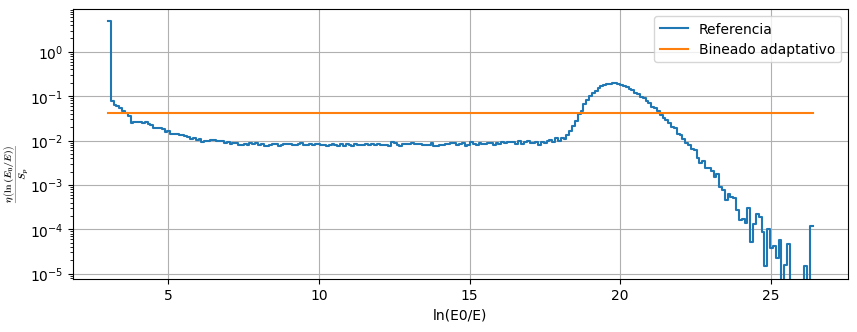
\includegraphics[width=\textwidth]{B_letargia_1.png}
    \caption{Distribución de letargía aproximada con un único bin. Se observa que el histograma es constante, representando el valor promedio sobre todo el dominio.}
    \label{fig:B_letargia_1}
\end{figure}

\begin{figure}[H]
    \centering
    \begin{subfigure}[b]{0.46\textwidth}
        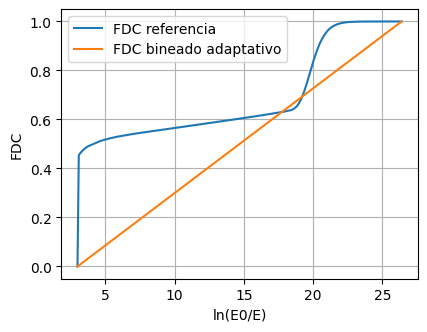
\includegraphics[width=\textwidth]{B_FDC_1.png}
        \caption{FDC original vs. FDC con 1 bin.}
        \label{fig:B_FDC_1}
    \end{subfigure}
    \hfill
    \begin{subfigure}[b]{0.46\textwidth}
        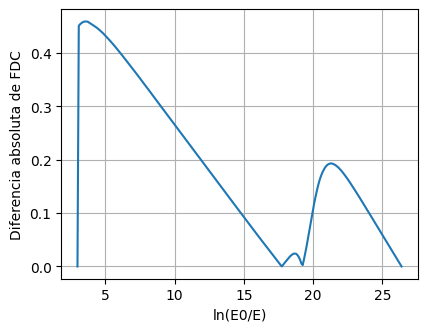
\includegraphics[width=\textwidth]{B_FDCdiff_1.png}
        \caption{Diferencia absoluta entre FDCs.}
        \label{fig:B_FDCdiff_1}
    \end{subfigure}
    \caption{Evaluación del criterio de refinamiento para el caso de 1 bin.}
    \label{fig:B_FDC_1_1}
\end{figure}

\section*{Caso con 2 bines}
\addcontentsline{toc}{section}{Caso con 2 bines}

En la Figura~\ref{fig:B_letargia_2} se muestra la distribución de letargía aproximada con 2 bines. En este caso, el histograma comienza a capturar la delta en $1~MeV$, pero con un bin de ancho considerable. En la Figura~\ref{fig:B_FDC_2} se presentan las FDCs de la distribución original de referencia y la obtenida con 2 bines, mientras que en la Figura~\ref{fig:B_FDCdiff_2} se muestra la diferencia absoluta entre ambas FDCs, que sirve como criterio para determinar la ubicación del nuevo bin en la siguiente iteración. Se observa que la posición del máximo en la Figura~\ref{fig:B_FDCdiff_2} ahora se encuentra con valor 0, producto de que se ubicó un bin en esa posición.

\begin{figure}[H]
    \centering
    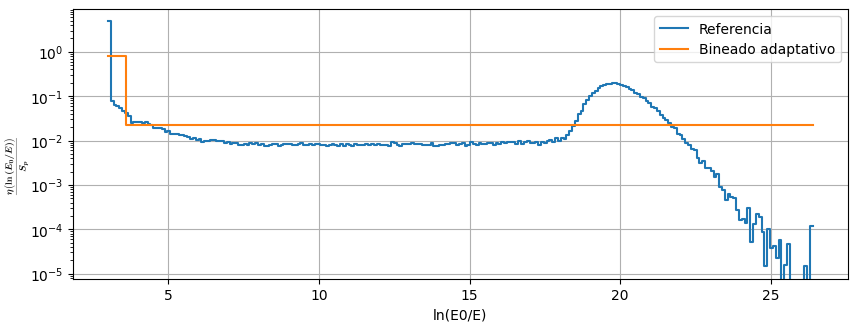
\includegraphics[width=\textwidth]{B_letargia_2.png}
    \caption{Distribución de letargía aproximada con 2 bines. Se observa que el método comienza a capturar la delta en $1~MeV$, pero con un bin de ancho considerable.}
    \label{fig:B_letargia_2}
\end{figure}

\begin{figure}[H]
    \centering
    \begin{subfigure}[b]{0.46\textwidth}
        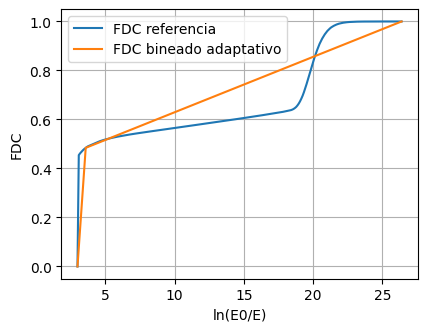
\includegraphics[width=\textwidth]{B_FDC_2.png}
        \caption{FDC original vs. FDC con 2 bines.}
        \label{fig:B_FDC_2}
    \end{subfigure}
    \hfill
    \begin{subfigure}[b]{0.46\textwidth}
        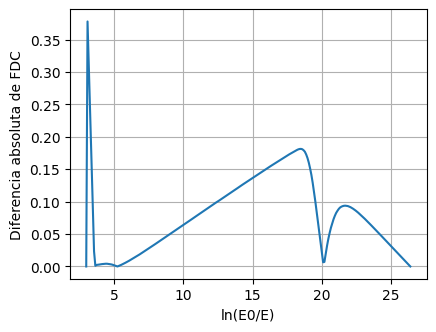
\includegraphics[width=\textwidth]{B_FDCdiff_2.png}
        \caption{Diferencia absoluta entre FDCs.}
        \label{fig:B_FDCdiff_2}
    \end{subfigure}
    \caption{Evaluación del criterio de refinamiento para el caso de 2 bines.}
    \label{fig:B_FDC_2_2}
\end{figure}

\section*{Caso con 3 bines}
\addcontentsline{toc}{section}{Caso con 3 bines}

En la Figura~\ref{fig:B_letargia_3} se muestra la distribución de letargía aproximada con 3 bines. En este caso, el histograma logra capturar la delta en $1~MeV$ con mayor precisión. En la Figura~\ref{fig:B_FDC_3} se presentan las FDCs de la distribución original de referencia y la obtenida con 3 bines, mientras que en la Figura~\ref{fig:B_FDCdiff_3} se muestra la diferencia absoluta entre ambas FDCs, que sirve como criterio para determinar la ubicación del nuevo bin en la siguiente iteración. \textbf{Nota para el corrector: aca en mas estoy repitiendo este parrafo para introducir las figuras y que no queden sin referencia. Podemos ver de cambiarlo si lo consideran necesario.}

\begin{figure}[H]
    \centering
    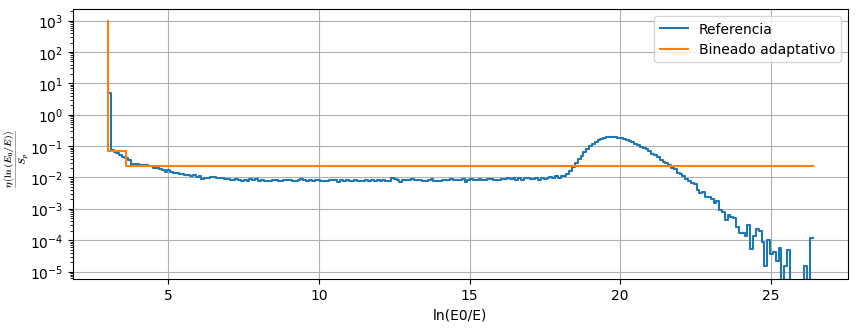
\includegraphics[width=\textwidth]{B_letargia_3.png}
    \caption{Distribución de letargía aproximada con 3 bines. Se observa que el método logra capturar la delta en $1~MeV$.}
    \label{fig:B_letargia_3}
\end{figure}

\begin{figure}[H]
    \centering
    \begin{subfigure}[b]{0.46\textwidth}
        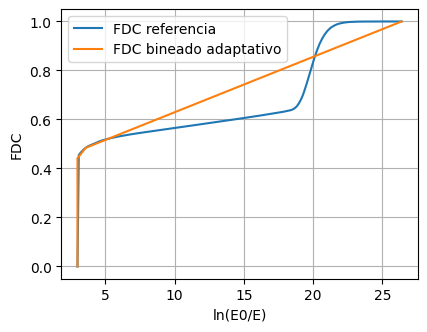
\includegraphics[width=\textwidth]{B_FDC_3.png}
        \caption{FDC original vs. FDC con 3 bines.}
        \label{fig:B_FDC_3}
    \end{subfigure}
    \hfill
    \begin{subfigure}[b]{0.46\textwidth}
        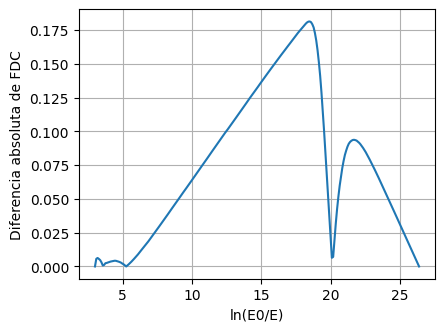
\includegraphics[width=\textwidth]{B_FDCdiff_3.png}
        \caption{Diferencia absoluta entre FDCs.}
        \label{fig:B_FDCdiff_3}
    \end{subfigure}
    \caption{Evaluación del criterio de refinamiento para el caso de 3 bines.}
    \label{fig:B_FDC_3_3}
\end{figure}

\section*{Caso con 5 bines}
\addcontentsline{toc}{section}{Caso con 5 bines}

En la Figura~\ref{fig:B_letargia_5} se muestra la distribución de letargía aproximada con 5 bines. En este caso, el histograma comienza a capturar la distribución en la región de termalización. En la Figura~\ref{fig:B_FDC_5} se presentan las FDCs de la distribución original de referencia y la obtenida con 5 bines, mientras que en la Figura~\ref{fig:B_FDCdiff_5} se muestra la diferencia absoluta entre ambas FDCs, que sirve como criterio para determinar la ubicación del nuevo bin en la siguiente iteración.

\begin{figure}[H]
    \centering
    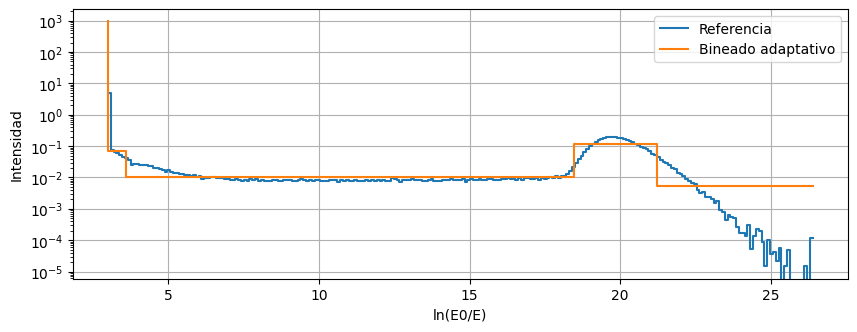
\includegraphics[width=\textwidth]{B_letargia_5.png}
    \caption{Distribución de letargía aproximada con 5 bines. Se observa que el método comienza a capturar la distribución en la región de termalización.}
    \label{fig:B_letargia_5}
\end{figure}

\begin{figure}[H]
    \centering
    \begin{subfigure}[b]{0.46\textwidth}
        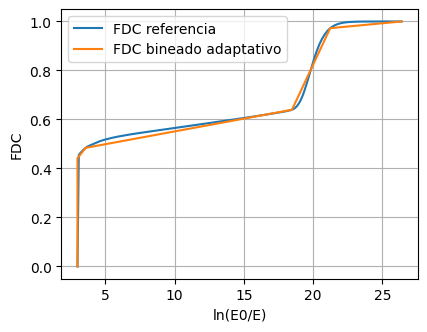
\includegraphics[width=\textwidth]{B_FDC_5.png}
        \caption{FDC original vs. FDC con 5 bines.}
        \label{fig:B_FDC_5}
    \end{subfigure}
    \hfill
    \begin{subfigure}[b]{0.46\textwidth}
        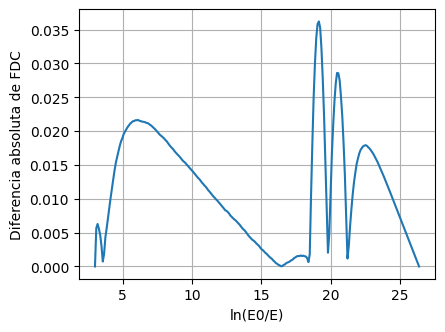
\includegraphics[width=\textwidth]{B_FDCdiff_5.png}
        \caption{Diferencia absoluta entre FDCs.}
        \label{fig:B_FDCdiff_5}
    \end{subfigure}
    \caption{Evaluación del criterio de refinamiento para el caso de 5 bines.}
    \label{fig:B_FDC_5_5}
\end{figure}

\section*{Caso con 10 bines}
\addcontentsline{toc}{section}{Caso con 10 bines}

En la Figura~\ref{fig:B_letargia_10} se muestra la distribución de letargía aproximada con 10 bines. En este caso, el histograma logra capturar la delta en $1~MeV$ y comienza a mejorar la aproximación de la distribución en la región de termalización y en la región epitérmica. En la Figura~\ref{fig:B_FDC_10} se presentan las FDCs de la distribución original de referencia y la obtenida con 10 bines, mientras que en la Figura~\ref{fig:B_FDCdiff_10} se muestra la diferencia absoluta entre ambas FDCs, que sirve como criterio para determinar la ubicación del nuevo bin en la siguiente iteración.

\begin{figure}[H]
    \centering
    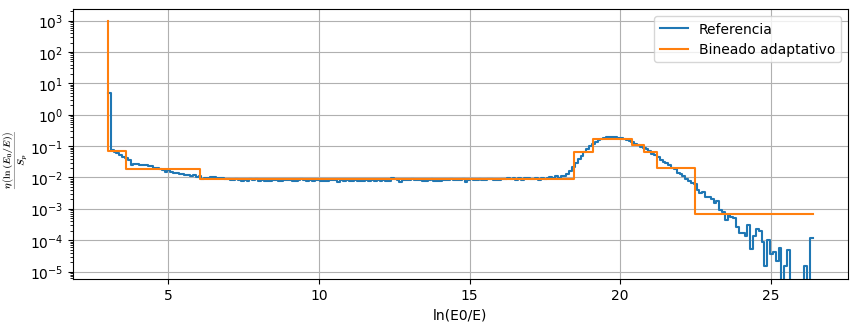
\includegraphics[width=\textwidth]{B_letargia_10.png}
    \caption{Distribución de letargía aproximada con 10 bines. Se observa que el método mejora la aproximación de la distribución en la región de termalización y en la región epitérmica.}
    \label{fig:B_letargia_10}
\end{figure}

\begin{figure}[H]
    \centering
    \begin{subfigure}[b]{0.46\textwidth}
        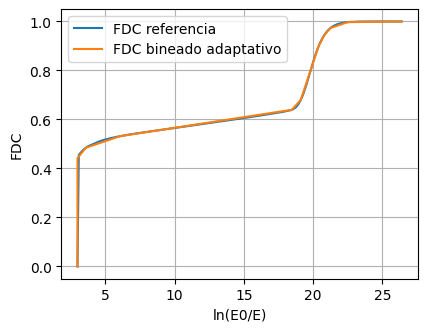
\includegraphics[width=\textwidth]{B_FDC_10.png}
        \caption{FDC original vs. FDC con 10 bines.}
        \label{fig:B_FDC_10}
    \end{subfigure}
    \hfill
    \begin{subfigure}[b]{0.46\textwidth}
        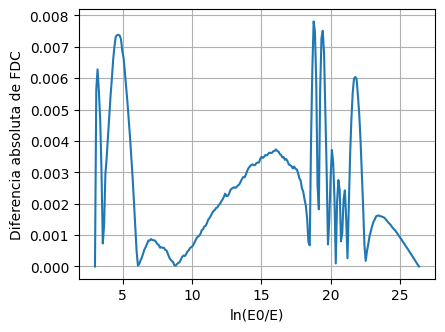
\includegraphics[width=\textwidth]{B_FDCdiff_10.png}
        \caption{Diferencia absoluta entre FDCs.}
        \label{fig:B_FDCdiff_10}
    \end{subfigure}
    \caption{Evaluación del criterio de refinamiento para el caso de 10 bines.}
    \label{fig:B_FDC_10_10}
\end{figure}

\section*{Caso con 25 bines}
\addcontentsline{toc}{section}{Caso con 25 bines}

En la Figura~\ref{fig:B_letargia_25} se muestra la distribución de letargía aproximada con 25 bines. En este caso, el histograma logra capturar la delta en $1~MeV$ y mejora significativamente la aproximación de la distribución en las regiones epitérmica y térmica, salvo para letargías mayores a \~ 22. En la Figura~\ref{fig:B_FDC_25} se presentan las FDCs de la distribución original de referencia y la obtenida con 25 bines, mientras que en la Figura~\ref{fig:B_FDCdiff_25} se muestra la diferencia absoluta entre ambas FDCs, que sirve como criterio para determinar la ubicación del nuevo bin en la siguiente iteración.

\begin{figure}[H]
    \centering
    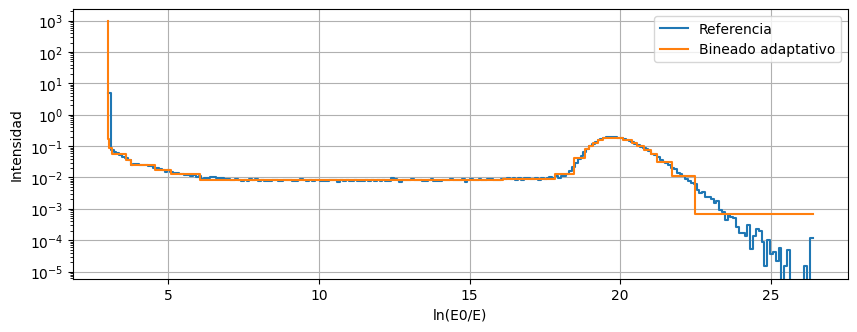
\includegraphics[width=\textwidth]{B_letargia_25.png}
    \caption{Distribución de letargía aproximada con 25 bines. Se observa que el método logra capturar la distribución de letargía, salvo en la región de letargía mayor a \~ 22, debido a la poca intensidad que tiene la distribución en esa región.}
    \label{fig:B_letargia_25}
\end{figure}

\begin{figure}[H]
    \centering
    \begin{subfigure}[b]{0.46\textwidth}
        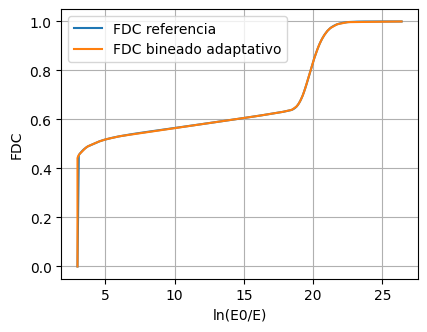
\includegraphics[width=\textwidth]{B_FDC_25.png}
        \caption{FDC original vs. FDC con 25 bines.}
        \label{fig:B_FDC_25}
    \end{subfigure}
    \hfill
    \begin{subfigure}[b]{0.46\textwidth}
        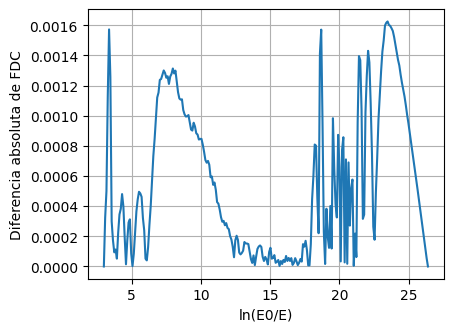
\includegraphics[width=\textwidth]{B_FDCdiff_25.png}
        \caption{Diferencia absoluta entre FDCs.}
        \label{fig:B_FDCdiff_25}
    \end{subfigure}
    \caption{Evaluación del criterio de refinamiento para el caso de 25 bines.}
    \label{fig:B_FDC_25_25}
\end{figure}

\section*{Caso con 100 bines}
\addcontentsline{toc}{section}{Caso con 100 bines}

En la Figura~\ref{fig:B_letargia_100} se muestra la distribución de letargía aproximada con 100 bines. En este caso, el histograma logra capturar con precisión la distribución de letargía, salvo en la región de letargía mayor a \~ 22, debido a la poca intensidad que tiene la distribución en esa región. Sin embargo se observa una mejoría con respecto al caso de 25 bines. En la Figura~\ref{fig:B_FDC_100} se presentan las FDCs de la distribución original de referencia y la obtenida con 100 bines, mientras que en la Figura~\ref{fig:B_FDCdiff_100} se muestra la diferencia absoluta entre ambas FDCs, que sirve como criterio para determinar la ubicación del nuevo bin en la siguiente iteración.


\begin{figure}[H]
    \centering
    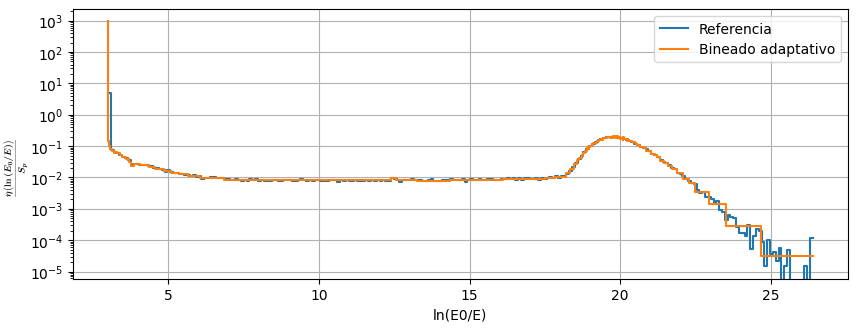
\includegraphics[width=\textwidth]{B_letargia_100.png}
    \caption{Distribución de letargía aproximada con 100 bines. Se observa que el método logra capturar con precisión la distribución de letargía, salvo en la región de letargía mayor a \~ 22, debido a la poca intensidad que tiene la distribución en esa región.}
    \label{fig:B_letargia_100}
\end{figure}

\begin{figure}[H]
    \centering
    \begin{subfigure}[b]{0.46\textwidth}
        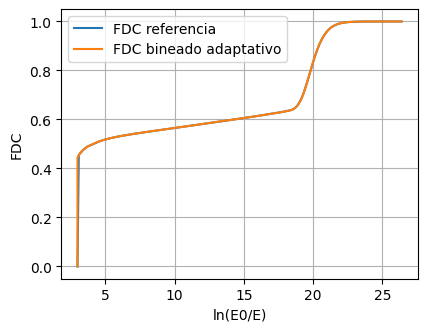
\includegraphics[width=\textwidth]{B_FDC_100.png}
        \caption{FDC original vs. FDC con 100 bines.}
        \label{fig:B_FDC_100}
    \end{subfigure}
    \hfill
    \begin{subfigure}[b]{0.46\textwidth}
        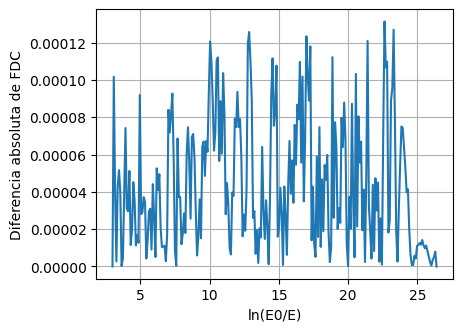
\includegraphics[width=\textwidth]{B_FDCdiff_100.png}
        \caption{Diferencia absoluta entre FDCs.}
        \label{fig:B_FDCdiff_100}
    \end{subfigure}
    \caption{Evaluación del criterio de refinamiento para el caso de 100 bines.}
    \label{fig:B_FDC_100_100}
\end{figure}





